\chapter{Background} \label{b}
% This section is an overview of arrows, multiparty session types (MPST) and free monad. Arrow is an interface of implicit data flow, and MPST can be used to describe explicit data flow. Free monad is a technique to convert normal DSL to a monadic DSL. 
As mentioned in the section \ref{i:m}, this section is an overview of a high-level language (section \ref{b:arrows} and \ref{b:pal}), from which a translation rule will be proposed to our intermediate languages, multiparty session types (section \ref{b:mpst}), the theoretical backbone giving rich features of the intermediate languages, and the free monad (section \ref{b:fm}), a technique in designing the intermediate languages.

\section{Arrows} \label{b:arrows}
Arrows, a general interface to describe computation, is the theoretical foundation of the high-level languages described in section \ref{b:pal}.
\subsection{Definition}
Definition of arrows will be represented in Haskell for convenience (shown in listing \ref{b:ar:c1}). In general, it can be defined in any programming language.

Intuitively, an arrow (y a b) can be regarded as computation from parameterised input a to parameterised output b. The simplest instance of arrow class is the basic function (shown in listing \ref{b:ar:c2}). Visually, arrows are like pipelines of computation with at least two inputs and at least two outputs (shown in figures \ref{b:ar:p1}\cite{HaskellUnderstandingArrows}). Programs formed by arrows are like compositions of pipelines.
\begin{code}
  % \inputminted{haskell}{background/ar-def.hs}
  \begin{minted}{haskell}
    class Arrow y where #\clabel{ar-def:1}#
      arr :: (a -> b) -> y a b
      first :: y a b -> y (a, c) (b, c)
      second :: y a b -> y (c, a) (c, b)
      (***) :: y a c -> y b d -> y (a, b) (c, d)
      (&&&) :: y a b -> y a c -> y a (b, c)
      (|||) :: y a c -> y b c -> y (Either a b) c  
  \end{minted}
  \ccaption{Arrow class in Haskell}{
    \begin{itemize}
      \item[\cref{ar-def:1}] Types of arrow functions 
    \end{itemize}
  }
  \label{b:ar:c1}
\end{code}
\begin{code}
  % \inputminted{haskell}{background/ar-func.hs}
  \begin{minted}{haskell}
    instance Arrow (->) where #\clabel{ar-func:1}#
      arr f = f
      (***) f g ~(x,y) = (f x, g y)
  \end{minted}
  \ccaption{$(\rightarrow)$ instance of Arrow class}{
    \begin{itemize}
      \item[\cref{ar-func:1}] Minimal implementation of arrow class are arr and ***
    \end{itemize}
  }
  \label{b:ar:c2}
\end{code}
\begin{figure*}
  \centering
  \begin{subfigure}[b]{0.475\textwidth}
      \centering
      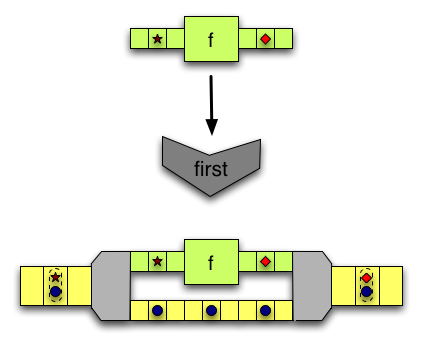
\includegraphics[width=\textwidth]{background/image/ArrowsConveyors_first2.png}
      % \caption{{\small Network 1}}    
      \label{fig:mean and std of net14}
  \end{subfigure}
  \hfill
  \begin{subfigure}[b]{0.475\textwidth}  
      \centering 
      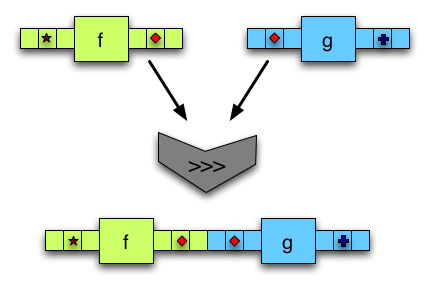
\includegraphics[width=\textwidth]{background/image/ArrowsConveyors_bind2.png}
      % \caption{{\small Network 2}}    
      \label{fig:mean and std of net24}
  \end{subfigure}
  \vskip\baselineskip
  \begin{subfigure}[b]{0.475\textwidth}   
      \centering 
      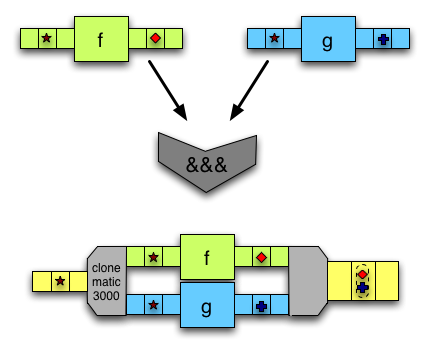
\includegraphics[width=\textwidth]{background/image/ArrowsConveyors_ampersand2.png}
      % \caption{{\small Network 3}}    
      \label{fig:mean and std of net34}
  \end{subfigure}
  \quad
  \begin{subfigure}[b]{0.475\textwidth}   
      \centering 
      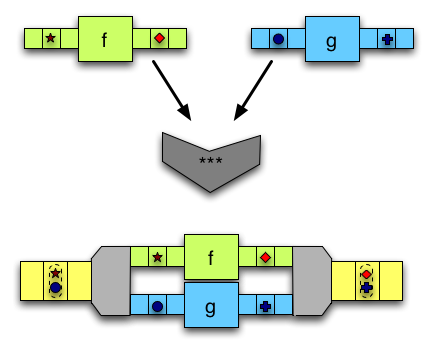
\includegraphics[width=\textwidth]{background/image/ArrowsConveyors_star2.png}
      % \caption{{\small Network 4}}    
      \label{fig:mean and std of net44}
  \end{subfigure}
  \caption
  {\small The visual representations of arrow combinatorcis}
  \label{b:ar:p1}
\end{figure*}
\subsection{Example: Calculate the mean}
Consider the a function to calculate the mean from a list of floating number, we will compare the usual implementation, implementations in arrows and point-free implementation.
\begin{minted}{haskell}
mean :: [Float] -> Float
mean xs = sum xs / (fromIntegral . length) xs

mean' :: [Float] -> Float
mean' = (sum &&& (length >>> fromIntegral)) >>> uncurry (/)

mean'' :: [Float] -> Float
mean'' = liftM2 (/) sum (fromIntegral . length)
\end{minted}
Above program can be visualized in figure \ref{b:ar:p2}.
\begin{figure}[ht]
  \centering
  \includegraphics[width=8cm]{example-image} 
  \caption{TODO: Add a visualization to show the pipelines}\label{b:ar:p2}
\end{figure}
The simple example demos that arrows combinatorcis make writing point-free programs easier. Arrows union the implementation of algorithm and data-flow in the algorithm. 

\subsection{Application in parallel computation}
From the previous example, the data flow of programs written regarding arrow combinators can be easily visualised. It is intuitive to recognise that the clean separation between the flow of data and computation will be useful in generating parallel codes. Indeed, arrow describes data flow implicitly, and it is an example of the so-called algebraic pattern. Many works (\cite{braunArrowsParallelComputation2018}, \cite{elliottGenericFunctionalParallel2017b} and \cite{authorAlgebraicMultipartyProtocol2018}) has been done to generate parallel codes from algebraic patterns.
In patricular, details of \cite{authorAlgebraicMultipartyProtocol2018} are introduced in section \ref{b:pal}.

\section{Multiparty session types} \label{b:mpst}
In complicated distributed systems, participants agree on a protocol, specifying type and direction of data exchanged. Multiparty session types are a branch of behavioural types specifically targeted at describing protocols in distributed systems based on asynchonous communication \cite{coppoGentleIntroductionMultiparty2015}. They're a type formalism used to model communication-based programming by codifying the structure of communication. The evolution of computing from the era of data processsing to the era of commucation witnessed the growth and significance of the theory of sesssion types.

The theory of multiparty session type contains three main elements. Global types (seen in section \ref{b:mpst:st}), local (session) types and processes. Processes are the concrete descriptions of the behaviour of the peers involed in the distributed system \cite{coppoGentleIntroductionMultiparty2015} using a formal language. Usually, the most used and the original langauge is $\pi$-calculus \cite{milnerCalculusMobileProcesses1992}. However, for the simplicity, we will not introduce $\pi$-calculus and use message passing primitives in Haskell (seen in section \label{b:mo:mpc}) instead. The coming sections are an intuitive introduction of session types by examples.
TODO: Add describtions about the MPST 1. describes explicit dataflow 2. so it can be used as the high-level programming languages to generate parallel codes 3. in section \ref{b:mpst:app}.
\subsection{Global types and local types} \label{b:mpst:st}
Global type is at the most abstract level, describing a communication protocol from a neutral viewpoing in terms of the interfactions that are supposed to occur between the protocol peers, of the order of these interactions, and of the kind of messages excahnged during these interactions \cite{coppoGentleIntroductionMultiparty2015}. The syntax of the global types is shwon in table \ref{b:mpst:gt} and an example of gloabl types is shown in \ref{b:mpst:gtex}.

Local types or session types characterise the same communication protocol as the global type, but from the viewpoint of each peer \cite{coppoGentleIntroductionMultiparty2015}. Each process is typed by local type. THe syntax of local types is shwon in table \ref{b:mpst:lt} and an example of local type is shown in \ref{b:mpst:ltex}. 

The relationship between global types and local types are established by the projection (seen in \ref{b:mpst:proj}) and a type system performs syntactic checks, ensuring that processes are typed by their corresponding local types. Hence, at the compile time, three important properties follows \cite{coppoGentleIntroductionMultiparty2015}. 
\begin{itemize}
  \item \textbf{communication safety}: Mismatches between the types of sent and expected messages, despite the same communication channel is used for excahnging messages of different types, do not exist \cite{coppoGentleIntroductionMultiparty2015}. 
  \item \textbf{protocol fidelity}: The interfactions that occurs are accounted for by the global type and therefore are allowed by the protocol \cite{coppoGentleIntroductionMultiparty2015}.
  \item \textbf{progress}: Every message sent is eventually received, and every process waiting for a message eventually receives one \cite{coppoGentleIntroductionMultiparty2015}.
\end{itemize}
We will learn that these properties are valuable not only in the distributed system but also in the domain of parallle computing in section \ref{b:mpst:app}.
% In the theory of multiparty session types, the whole distributed system is described by global types representing the communication protocols from a global viewpoint.  Each process are typed by local types which characterise the same communication protocols as global types but from a perspective of individual participants \cite{coppoGentleIntroductionMultiparty2015}.
\begin{table}[ht]
\centering
\begin{grammar}{G\Coloneqq}{Global types}
  p \rightarrow q : \langle S \rangle.G & Value exchange \\
  p \rightarrow q : \langle T \rangle.G & Channel exchange \\
  p \rightarrow q : \{ l_i : G_i \}_{i \in I} & Bracnhing \\
  \mu \mathbf{t}.G  \mid \mathbf{t} \mid \text{end} & Recursion/End
\end{grammar}
\caption{Global types} \label{b:mpst:gt}
\end{table}
\begin{table}[ht]
\begin{grammar}{S\Coloneqq}{Sorts}
  \text{bool} \mid \text{nat} \mid \text{string} \\
  \dots\\
\end{grammar}
% \begin{grammar}{T\Coloneqq}{Session types/local types}
%   ! \langle p, S \rangle . T & Send value\\
%   ! \langle p, T \rangle . T & Send channel\\
%   ? ( p, T ) . T & Channel Receive\\
%   ? ( p, S ) . T & Sorts Receive\\
%   \oplus \langle p, \{ l_i : T_i \}_{i \in I} \rangle & Selection \\
%   \&(p, \{l_i : T_i \}_{i \in I}) & Bracnhing \\
%   \mu \mathbf{t}.T  \mid \mathbf{t} \mid \text{end} & Recursion/End
% \end{grammar}
\hfill
\begin{grammar}{T\Coloneqq}{Session types/local types}
  ! \langle p, S \rangle . T & Send value\\
  ! \langle p, T \rangle . T & Send channel\\
  ? ( p, T ) . T & Channel Receive\\
  ? ( p, S ) . T & Sorts Receive\\
  \oplus \langle p, \{ l_i : T_i \}_{i \in I} \rangle & Selection \\
  \&(p, \{l_i : T_i \}_{i \in I}) & Bracnhing \\
  \mu \mathbf{t}.T  \mid \mathbf{t} \mid \text{end} & Recursion/End
\end{grammar}
\caption{Session types/local types} \label{b:mpst:lt}
\end{table}[ht]
\begin{table}
  \begin{minipage}{0.45\textwidth}
    \begin{enumerate}
      \item Customer(0) sends an order number to Agency(1) and Agency sends back a quote to customer.
      \item If Customer is happy with the price then Customer selects accept option and notifies Agency.
      \item If Customer thinks the price is too high then Customer terminate the trade by selecting reject.
      \item If accept is selected, Agency notify both Customer and Agency2(2). 
      \item Customer sends an address to Agency2 and Agency2 sends back a deliver date.
    \end{enumerate}
  \end{minipage}
  \hfill
  \begin{minipage}{0.45\textwidth}
    \begin{align*}
      G = \\
      & 0 \rightarrow 1: && \langle \text{string} \rangle .\\
      & 1 \rightarrow 0: && \langle \text{int} \rangle .\\
      & 0 \rightarrow 1: \{ && \text{accept}: \\
      & && 1 \rightarrow \{ 0, 2 \}: \langle \text{string} \rangle . \\
      & &&  0 \rightarrow 2: \langle \text{string} \rangle .\\
      & &&  2 \rightarrow 0: \langle \text{int} \rangle . \text{end}, \\
      & && \text{reject}: \text{end} \} \\
    \end{align*}
  \end{minipage}
  \caption{An example of protocal described by global types G}
  \label{b:mpst:gtex}
\end{table}
\begin{table}[ht]
  \begin{minipage}{0.45\textwidth}
    \begin{align*}
      S \triangleq \mu t.(\&\{ & \text{balance}: ![\text{nat}];t, \\
        & \text{deposit}: ?[\text{nat}];![\text{nat}];t, \\
        & \text{exit}: \text{end}\}) \\
    \end{align*}
  \end{minipage}
  \hfill
  \begin{minipage}{0.45\textwidth}
    \begin{align*}
      C \triangleq \oplus \{ &\text{balance}: ?[\text{nat}];\text{end}, \\
                             &\text{deposit}: ![\text{nat}];?[\text{nat}];\text{end} \} 
    \end{align*}
  \end{minipage}
  \caption{Session types of client and server end point of a ATM service}
  \label{b:mpst:ltex}
\end{table}
\subsubsection{Projection between global types and local types} \label{b:mpst:proj}
Projection is the formalisation of the relationship between global and local types. It's an operation extracting the local type of each peer from the global type \cite{coppoGentleIntroductionMultiparty2015}. The definition of projection is shown in table \ref{b:mpst:pdef}.

As an example, a projection of global type in table \ref{b:mpst:gtex} is
$$
  G \upharpoonright 0 = !\langle 1, \text{string} \rangle;?(1, \text{string});\&(1, \{ \text{accept}: ?(1, \text{string});!\langle 2, \text{string} \rangle;?(2, \text{int}), 
  \text{reject}: \text{end} \})
$$  
\begin{table}[H]
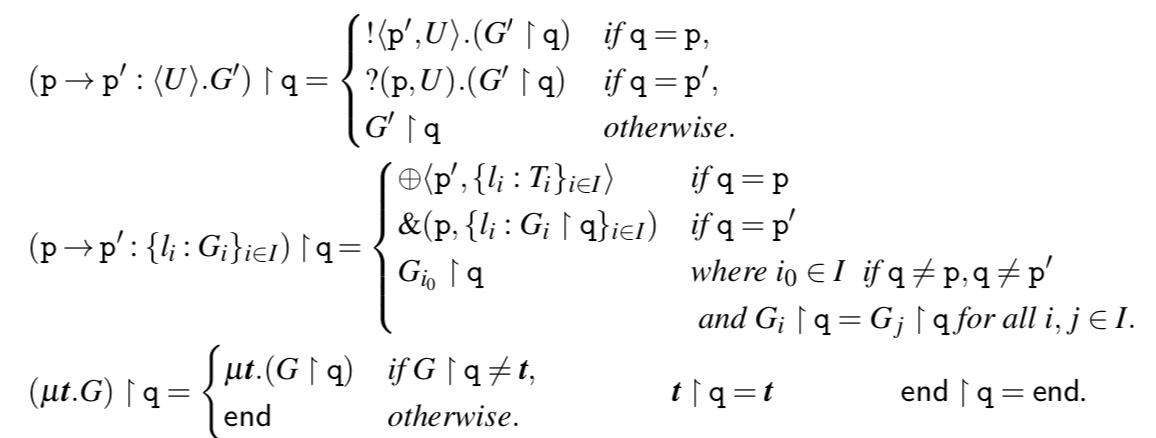
\includegraphics[width=\textwidth]{background/image/proj-def.png}
\caption{The definition of projection of a global type G onto a participants q\cite{coppoGentleIntroductionMultiparty2015}}
\label{b:mpst:pdef}
\end{table}
\subsubsection{Duality of session types}
In binary session types where all protocals are pairwise, duality formalise the relationship between the types of opposite endpoints. For a type $T$, its dual or co type, written $\bar{T}$ is defined inductively as in table \ref{b:mpst:dualdef}.
\begin{table}[H]
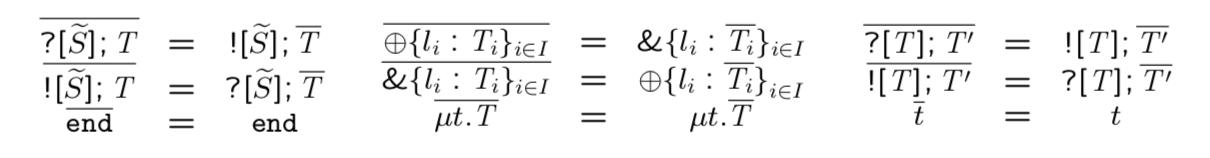
\includegraphics[width=\textwidth]{background/image/dual-def.png}
\caption{Inductive definition of duality}
\label{b:mpst:dualdef}
\end{table}

Duality is essential for checking type compatability. Compatible types mean that each common channel $k$ is associated with complementary behaviour: this ensures that the interactions on $k$ run without erros. 

In order to apply duality into multiparty session types in which more than two participants are allowed, we introduce the partial projection (seen in \cite{coppoGentleIntroductionMultiparty2015}) from multiparty session type to binary session type so that we can resue the definition of duality after applying the partial projection.
% \begin{table}[H]
% \caption{The pa}
% \label{b:mpst:partproj}
% \end{table}
% \begin{table}[ht]
% \begin{align*}
% \end{align*}
% \caption{Inductive definition of duality} \label{b:mpst:dual}
% \end{table}
\subsection{Example: arithmetic server}
\subsection{Applications in parallel computing} \label{b:mpst:app}
Multiparty session types not only have rich applications in distributed systems but also value in the domain of parallel computation. 

Existing work\cite{ngSafeMPICode} has shown how to generate MPI\footnote{Message Passing Interface (MPI) is a standardised and portable message-passing standard designed by a group of researchers from academia and industry to function on a wide variety of parallel computing architectures \cite{MessagePassingInterface2018}.} programs using session types. Users describe the communication topology as a skeleton using a protocol language which is type checked by session types. After that, an MPI program is generated by merging the skeleton and user-provided kernels for each peer. The parallel codes obtained in this way is guaranteed to be deadlock-free and progressing. 

\section{Message passing concurrency}
This section introduce some interfaces for message passing concurrency from the primitive case: channel to more advanced one: monad for message passing concurrency.

For the simplicity, they're represented in Hasekll but in general most languages can implement similar interfaces. 
\subsection{Primitives for message-passing concurrency} \label{b:mo:mpc}
In section \ref{b:mpst}, channels are bi-directional and used for communication between two parties. In Haskell, channel primitives are represented in listing \ref{b:mo:c1}. However, just using these primitives cannot guarantee progress or communication safety. For example, a program that has one thread writing channel once combined with another thread reading channel twice is type-correct but will cause deadlock. Many kinds of research to encode MPST using Haskell's type system are presented in \cite{orchardSessionTypesLinearity} so that an (MPST) type-correct Haskell program assures progress, communication safety and session fidelity.
\begin{listing}[ht]
  \inputminted{haskell}{background/mo-chan.hs}
  \caption{Channel primitives in Haskell}
  \label{b:mo:c1}
\end{listing}
\subsection{Concurrency Monads}
The work done by \cite{claessenFunctionalPearlsPoor1999} constructs a monad to express concurrent computation. The definition is in listing \ref{b:mo:c2}. The idea is using continuation to represent the "future" so that computation can pause and resume as well as expressing sequential computation. Atom wraps the actual computation and Fork is responsible for spawning threads. Monad encapsulates the continuation and makes writing program compositionally in a monadic way.

\begin{code}
  % \inputminted{haskell}{background/mo-cm.hs}
  \begin{minted}{haskell}
    data Action =          #\clabel{mo-cm:1}#
        Atom (IO Action)   #\clabel{mo-cm:2}# 
      | Fork Action Action #\clabel{mo-cm:3}# 
      | Stop               #\clabel{mo-cm:4}# 
    
    newtype C a = C { runC :: (a -> Action) -> Action } #\clabel{mo-cm:5}#
    
    instance Monad C where
        (>>=) :: C a -> (a -> C b) -> C b #\clabel{mo-cm:6}#
        m >>= f  = C $ \k -> runC m (\v -> runC (f v) k)
        return :: a -> C a
        return x = C $ \k -> k x
    
    schedule :: [Action] -> IO () #\clabel{mo-cm:7}#
    schedule [] = return ()
    schedule (a:as) = sched as a
    
    sched :: [Action] -> Action -> IO ()
    sched as (Atom ioa) = do
        a <- ioa
        schedule $ as ++ [a] 
    sched as (Fork a1 a2) = schedule $ as ++ [a2, a1]
    sched as Stop = schedule as
    
    atom :: IO a -> C a #\clabel{mo-cm:8}#
    atom m = C $ \k -> Atom $ do
        r <- m
        return $ k r
    
    fork :: C () -> C ()
    fork m = C $ \k -> Fork (runC m (const Stop)) (k ())
  \end{minted}
  \ccaption{Concurrency Monads and sequential scheduler}{
    \begin{itemize}
      \item[\cref{mo-cm:1}] Basic unit of computation : Action. A program is the composition of Actions.
      \item[\cref{mo-cm:2}] Atom is a IO computation followed by an action.
      \item[\cref{mo-cm:3}] Fork is two 'parallel' action.
      \item[\cref{mo-cm:4}] Stop is the termination of an action.
      \item[\cref{mo-cm:5}] Using a monad C to encapsulates continuation
      \item[\cref{mo-cm:6}] Monad bind is used to represent sequence of Actions.
      \item[\cref{mo-cm:7}] An implementation of a sequential scheduler. sched is the helper function.
      \item[\cref{mo-cm:8}] atom and fork are combinators to compose programs.
    \end{itemize}      
  }
  \label{b:mo:c2}
\end{code}

\begin{code}
\begin{minted}{haskell}
example :: C ()
example = do 
    atom $ putStrLn "Hello" 
    name <- atom getLine 
    fork $ atom $ putStrLn "World"
    atom $ putStrLn name
\end{minted}
\caption{Example of a program writen in concurrency monad}
\end{code}

It is worth mentioning that the concurrency monad can be extended to support many features. For example, work done by \cite{marlowMonadDeterministicParallelism} modifies the definition of Action as. well as implements a work-stealing parallel scheduler (seen in listing \ref{b:mo:c3}) to build a monad for parallel computation. 

Besides, Extending the concurrency monad to monad for message-passing concurrency can be done by adding channel primitives like newChan, writeChan and readChan into the Action.. Since channel primitives are possible to represent in this monad, we naturally think of its prospect in connecting with MPST (will be discussed in the later section).
\begin{code}
  % \inputminted{haskell}{background/mo-par.hs}
  \begin{minted}{haskell}
    newtype IVar a = IVar (IORef (IVarContents a)) #\clabel{po:ivar}#
    data IVarContents a = Full a | Blocked [a -> Action.]
    
    data Action .=
        Fork Action Action
      | Stop
      | forall a . Get (IVar a) (a -> Action) #\clabel{po:get}#
      | forall a . Put (IVar a) a Action #\clabel{po:put}#
      | forall a . New (IVar a -> Action)
  \end{minted}
%   \caption[.]{
%   \begin{minipage}{\linewidth}
%     Par Monad
%     \begin{itemize}
%       \item[\cref{mylin2} :] hello 
%       \item[\cref{mylin2} :] hello 
%     \end{itemize}
%     % \begin{align*}
%       % x &= y\\ 
%       % x &= x + 1\\ 
%       % x &= 0\\
%     % \end{align*}
%  \end{minipage}
%  }
  \ccaption{Par Monad}{
    \begin{itemize}
      \item[\cref{po:ivar}] Parent threads and child threads communicate data via IVar
      \item[\cref{po:get}] Get operation blocks when the underlying IVarContents is Blocked  
      \item[\cref{po:put}] Put operation updates the underlying IVarContetns to Full with the result a and resume the list of blocking threads by applying a to the continuation.
    \end{itemize}
  }
  \label{b:mo:c3}
\end{code}

In summary, many techniques and ideas like continuation presented in the implementation of this monad afford us inspirations in designing the intermediate language.
\section{Free monad} \label{b:fm}
Free monad \footnote{The mathematical definition of the free monad can be found in \cite{contributorsCatsFreeMonads}} is a concept from category theory.
% \footnote{Free monad is a construction that is left adjoint to a forgetful functor whose domain is the category of Monads and whose co-domain is the category of Endofunctors \cite{contributorsCatsFreeMonads}. Intuitively, it says any functor can construct a monad}. 
Functional programming language exploits this concept because of its applications in domain specific language, especially in interpreters (section \ref{b:fm:a}).
\subsection{Definition}
In practice, a free monad in Haskell can be defined as an algebraic data type(ADT). As promised in category theory, it is an instance of monad type class given f is a functor (shown in listing \ref{b:fm:c1}). Many useful helper functions are derived from the simple definition of the free monad (shown in listing \ref{b:fm:c2}).
\begin{code}
  \inputminted{haskell}{background/fm-construction.hs}
  \caption{Free monad in Haskell}
  \label{b:fm:c1}
\end{code}
\begin{code}
  \inputminted{haskell}{background/fm-helper.hs}
  \caption{Helper functions based on free monad}
  \label{b:fm:c2}
\end{code}
\subsection{Example} \label{b:fm:e}
As mentioned, free monad is useful in interpreting an abstract syntax tree (AST). In order to apply free monad to a given AST, we can follow a routine \cite{contributorsCatsFreeMonads}.
\begin{enumerate}
  \item Create an AST, usually represented as an ADT
  \item Implement functor for the ADT
  \item Create helper constructors to Free ADT for each type constructor in ADT by liftF 
  \item Write a monadic program using helper constructors. It is essentially a program written in DSL operations.
  \item Build interpreters for Free ADT by interpreting
  \item Interpret the program by the interpreter.
\end{enumerate}
We will demo the above procedure by a made-up example. First of all, we create a simple AST in ADT. 
\begin{code}
\begin{minted}{haskell}
data GreetingF next
  = Getname (String -> next)
  | Greet String next
  deriving Functor

type Greeting = Free GreetingF
\end{minted}
% \caption[.]{
%   \begin{minipage}{\linewidth}
%     Par monad
%     \begin{itemize}
%       \item[\cref{mylin2} :] hello 
%       \item[\cref{mylin2} :] hello 
%     \end{itemize}
%  \end{minipage}
%  }
\end{code}
Then we create helper constructors of Greeting using liftF.
\begin{minted}{haskell}
getName = liftF $ Getname id
greet str = liftF $ Greet str ()
\end{minted}
Then we can write a simple program using operations provided by Greeting.
\begin{minted}{haskell}
exampleProgram :: Greeting ()
exampleProgram = do
    a <- getName
    greet a
    b <- getName
    greet b
\end{minted}
Then we can easily implement an interpreter for the example program
\begin{minted}{haskell}
goodMorningInterpreter :: Greeting a -> IO a
goodMorningInterpreter = interpret helper
    where
        helper (Getname next) = fmap next getLine
        helper (Greet str next) = putStrLn ("Good morning " ++ str) >> return next  
\end{minted} 
Finally, execute the program.
\begin{minted}{bash}
ghci:> goodMorningInterpreter exampleProgram
Tom
Good morning Tom
Mary
Good morning Mary
\end{minted}
% \begin{listing}
%   \inputminted{haskell}{background/fm-example.hs}
%   \caption{An example of free moand}
%   \label{b:fm:c3}
% \end{code}

\subsection{Applications} \label{b:fm:a}
As illustrated by the example (section \ref{b:fm:e}), free monad decouple the abstract syntax tree of domain specific language (DSL) and the interpreter. Interpreters with different purposes can be implemented without changing the syntax.

In the project, we apply free monad to the intermediate language so not only we make the languages monadic for free but also benefits from decoupling the interpreter and the syntax to implement different interpreters, e.g. Simulator, code generators to different platforms easily.
\section{Summary}